%!TEX root = ../thesis.tex

\thispagestyle{myheadings}
\graphicspath{{Body/Figures/Theory/}}

\chapter{Introduction}
\label{chapter:Introduction}

The prevailing theory for particle physics, the Standard Model (SM), has had tremendous success in describing our universe. It has been used to predict and explain a wide variety of phenomena and particles, their properties and interactions, to great precision. However, in spite of its success in explaining nearly all experimental results, there exist unanswered questions about our universe. Some of these include the matter-antimatter asymmetry, the source of mass for the neutrinos, the existence of dark matter, and an inability to fully incorporate our best theory of gravitation. Many particle physics experiments are being devised and conducted around the world in order to shed light on these questions and improve our understanding of reality. One such particular experiment is the Fermilab Muon \gmtwo Experiment (E989) underway at the Fermi National Accelerator Laboratory (FNAL) located in Batavia, Illinois.

I have been a part of the E989 experiment since I began my graduate degree six years ago. Three years ago I moved from Boston to Batavia to be where the action is. This dissertation will describe in detail the work which I have done for the experiment. Chapter 1 will provide experimental and theoretical background to the experiment, as well its motivation. Chapter 2 will  describe the experimental principle. Chapter 3 will describe the magnetic field portion of the experiment, and magnetic field simulations I conducted. Chapter 4 will describe the straw tracking detectors and their measurements, including the track fitting I wrote. Chapter 5 will describe the frequency measurement portion of the experiment, and detail the analysis results from data taken in the first half of 2018. Finally, Chapter 6 will concluded the thesis and the important results contained within.


\section{Magnetic Dipole Moments}
\label{sec:MDMs}

In order to understand the purpose of the Fermilab Muon \gmtwo Experiment, first we need to understand what the $g$ in \gmtwo is, which is what the experiment is measuring. All particles have intrinsic properties which describe those particles. One of those properties is the so called magnetic dipole moment. This property of a particle is related to its spin through the equation
		\begin{align}
            \vec{\mu} = g \frac{Qe}{2m} \vec{s},
        \label{eq:magneticmoment}
		\end{align}
where $\vec{\mu}$ is the magnetic dipole moment of a particle, $\vec{s}$ is its spin vector, $m$ is its mass, $e$ is the elementary charge, $Q = \pm1$, and \g is the so called "g-factor". (Here and following $c$ and $\hbar$ have been set to 1.) \g is some measureable and predictable constant, which as shown in \equref{eq:magneticmoment} simply relates the magnetic moment of a particle to its spin angular momentum. 

In a Dirac theory, \g is equal to 2 for spin-1/2 particles with no internal structure \cite{Dirac}. See Appendix~\ref{gDirac} for a derivation of this result. It turns out however, that \g is not quite equal to 2 even for these types of simple particles. Motivated by early experimental discrepencies such as the measurements of the hyperfine structure in hydrogen \cite{EarlyHyperfine1}, in 1948 Schwinger calculated the first "radiative correction" to the electron magnetic moment \cite{Schwinger}. In a quantum field theory, interactions of the particle with virtual particles in loops will contribute to the value of \g. In this context it is nicer to recast the magnetic moment formula as 
		\begin{equation}
		\begin{aligned}
            \vec{\mu} &= 2(1+a) \frac{Qe}{2m} \vec{s}, \\
            a &= \frac{g-2}{2},
        \label{eq:anamoly}
		\end{aligned}
		\end{equation}
where $a$ is called the "anamolous" part of the magnetic moment, and contains all higher order corrections. The first correction calculated to $a$ by Schwinger was $a = \alpha/2\pi \approx 0.00116$, where $\alpha$ is the fine structure constant. By measuring $a$, the SM theory (and extensions to it) can be tested. The measurement of the anamolous piece of the muon is indeed where the Fermilab Muon \gmtwo Experiment gets its name.


\subsection{Why the muon and not the electron?}

The magnetic moment of the electron has been measured extraordinarily precisely, to .28 parts per trillion (ppt) \cite{ElectronMDM}. It has been used to test SM theory extensively, and specifically the QED portion of it. Because the electron is so light, the contributions to $a_{e}$ come almost exclusively from QED. This is because the various contributions from both the weak and hadronic sectors contain couplings which depend on the mass of the particle squared. It is for this reason that the magnetic moment of the muon is such an interesting quantity to measure. Since the muon is approximately 200 times heavier than the electron, the senstivity of \amu to radiative corrections is approximately 4000 times greater than that for the the electron.


\section{Standard Model Contributions to \amu}
\label{sec:Theory}


Before experimental results have any real meaning, they need a theory with which to compare. The latest theoretical predictions for the muon magnetic moment will be presented here. The contributions to \amu can be summed from separate pieces relating to different parts of the SM. These include the quantum-electrodynamics (QED) corrections purely from other leptons and photons, the electroweak (EW) corrections from interactions with the weak force bosons $W^{\pm}$ and $Z^{0}$, and the hadronic corrections from interactions with hadrons: 
		\begin{align}
            a_{\mu}^{\text{SM}} = a_{\mu}^{\text{QED}} + a_{\mu}^{\text{EW}} + a_{\mu}^{\text{Had}}
		\end{align}
The QED corrections are very well understood and have been calculated to very high order. The electroweak corrections are harder to calculate, but due to the heavy masses of the force carrying bosons and by extension weaker couplings, are only required to be known up to two loop level. And indeed they are. Finally, the hadronic contributions are where most of the theoretical uncertainties lie, and where most active work is going on. Indeed there are also some data-driven approaches to the hadronic contributions which are interesting and will be discussed in a following section.






-just put words down on the page, keep it short and simple, I can go back and add detail where necessary, I'll have to do a lot of editing anyways
-dont worry about the ordering of sections exactly either
-check Saskia's thesis for the latest theoretical results


- see papers cited in my HEP2 class paper - and then look for new ones
- Fred Jegerlehner's book




\subsection{QED}
\label{subsec:QED}

The QED contributions to \amu stem solely from loops with virtual leptons and photons. They have been calculated up to 5 loop levels from over 12,000 Feynman diagrams \cite{Kinoshita1,Kinoshita2}. The first couple of diagrams including the Dirac $g = 2$ and Schwinger diagrams are shown in \figref{fig:QEDDiagrams}. The value is
		\begin{align}
            a_{\mu}^{\text{QED}} = (11658471.8971 \pm 0.007) \times 10^{10}.
		\end{align}
Over 99\% of the value of \amu comes from the QED parts, but the error is much smaller than the other contributions and than the experimental uncertainty.

\begin{figure}[]
\centering
	\begin{subfigure}[t]{0.3\textwidth}
	\centering
		\begin{tikzpicture}[baseline=(o.base)]
		\begin{feynhand}
		\large
		\setlength{\feynhandlinesize}{1pt}
		\vertex [dot] (o) at (0,0);
		\vertex (a) at (-2,-2) {$l$}; 
		\vertex (b) at (2,-2) {$\overline l$}; 
		\vertex (c) at (0,2) {B};
		\propag [fermion] (a) to (o);
		\propag [anti fermion] (b) to (o);
		\propag [photon] (c) to [edge label = $\gamma$] (o);
		\end{feynhand}
		\end{tikzpicture}
	\caption{Dirac result, $g=2$.}
	\end{subfigure}
	\hspace{3mm}
	\begin{subfigure}[t]{0.3\textwidth}
	\centering
		\begin{tikzpicture}[baseline=(o.base)]
		\begin{feynhand}
		\large
		\setlength{\feynhandlinesize}{1pt}
		\vertex [dot] (o) at (0,0);
		\vertex (a) at (-2,-2) {$l$}; 
		\vertex (b) at (2,-2) {$\overline l$}; 
		\vertex (c) at (0,2) {B};
		\vertex (d) at (-1,-1);
		\vertex (e) at (1,-1);
		\propag [fermion] (a) to (d);
		\propag [fermion] (d) to (o);
		\propag [anti fermion] (b) to (e);
		\propag [anti fermion] (e) to (o);
		\propag [photon] (c) to [edge label = $\gamma$] (o);
		\propag [photon] (d) to [edge label' = $\gamma$] (e);
		\end{feynhand}
		\end{tikzpicture}
	\caption{The first loop diagram, calculated by Schwinger.}
	\end{subfigure}
	\hspace{3mm}
	\begin{subfigure}[t]{0.3\textwidth}
	\centering
		\begin{tikzpicture}[baseline=(o.base)]
		\begin{feynhand}
		\large
		\setlength{\feynhandlinesize}{1pt}
		\vertex [dot] (o) at (0,0);
		\vertex (a) at (-2,-2) {$l$}; 
		\vertex (b) at (2,-2) {$\overline l$}; 
		\vertex (c) at (0,2) {B};
		\vertex (d) at (-1,-1);
		\vertex (e) at (1,-1);
		\vertex (f) at (-.5,-1);
		\vertex (g) at (+.5,-1);
		\propag [fermion] (a) to (d);
		\propag [fermion] (d) to (o);
		\propag [anti fermion] (b) to (e);
		\propag [anti fermion] (e) to (o);
		\propag [photon] (c) to [edge label = $\gamma$] (o);
		\small
		\propag [boson] (d) to [edge label' = $\gamma$] (f);
		\propag [boson] (g) to (e);
		\propag [fermion] (f) to [half left, edge label = $l$] (g);
		\propag [anti fermion] (f) to [half right, edge label' = $\overline l$] (g);
		\end{feynhand}
		\end{tikzpicture}
	\caption{A two loop diagram.}
	\end{subfigure}
\caption[QEDDiagrams]{The first of many QED diagrams contributing to $a$. B is a magnetic field. Feynman diagrams made with \cite{tikz-feynman,tikz-feynhand}.}	
\label{fig:QEDDiagrams}
\end{figure}



\subsection{Electroweak}
\label{subsec:Electroweak}

The electroweak contributions to \amu are known to two loop level, with some 3 loop parts estimated. The contributions stem from couplings with the heavy weak gauge bosons. Because the couplings to these heavy bosons are small, the electroweak contributions to \amu are small. The different one loop diagrams and an example two loop diagram are shown in \figref{fig:EWDiagrams}. The value of the elctroweak contributions is
		\begin{align}
            a_{\mu}^{\text{EW}} = (15.12 \pm 0.1) \times 10^{10}.
		\end{align}
with improvements having been made recently \cite{EW1,EW2}. Again the error on these contibutions are small compared to the hadronic contributions discussed next, as well as the experimental uncertainties.


\begin{figure}[]
\centering
	\begin{subfigure}[t]{0.3\textwidth}
	\centering
		\begin{tikzpicture}[baseline=(o.base)]
		\begin{feynhand}
		\large
		\setlength{\feynhandlinesize}{1pt}
		\vertex [dot] (o) at (0,0);
		\vertex (a) at (-2,-2) {$l$}; 
		\vertex (b) at (2,-2) {$\overline l$}; 
		\vertex (c) at (0,2) {B};
		\vertex (d) at (-1,-1);
		\vertex (e) at (1,-1);
		\propag [fermion] (a) to (d);
		\propag [fermion] (d) to (o);
		\propag [anti fermion] (b) to (e);
		\propag [anti fermion] (e) to (o);
		\propag [photon] (c) to [edge label = $\gamma$] (o);
		\propag [boson] (d) to [edge label' = $Z^{0}$] (e);
		\end{feynhand}
		\end{tikzpicture}
	\caption{Exchange of a virtual $Z^{0}$ boson.}
	\end{subfigure}
	\hspace{3mm}
	\begin{subfigure}[t]{0.3\textwidth}
	\centering
		\begin{tikzpicture}[baseline=(o.base)]
		\begin{feynhand}
		\large
		\setlength{\feynhandlinesize}{1pt}
		\vertex [dot] (o) at (0,0);
		\vertex (a) at (-2,-2) {$l$}; 
		\vertex (b) at (2,-2) {$\overline l$}; 
		\vertex (c) at (0,2) {B};
		\vertex (d) at (-1,-1);
		\vertex (e) at (1,-1);
		\propag [fermion] (a) to (d);
		\propag [anti fermion] (b) to (e);
		\propag [photon] (c) to [edge label = $\gamma$] (o);
		\propag [fermion] (d) to [edge label' = $\overline \nu_{l}$] (e);
		\small
		\propag [boson] (d) to [edge label = $W^{-}$] (o);
		\propag [boson] (e) to [edge label' = $W^{+}$] (o);
		\end{feynhand}
		\end{tikzpicture}
	\caption{Weak loop with $W$ bosons.}
	\end{subfigure}
	\hspace{3mm}
	\begin{subfigure}[t]{0.3\textwidth}
	\centering
		\begin{tikzpicture}[baseline=(o.base)]
		\begin{feynhand}
		\large
		\setlength{\feynhandlinesize}{1pt}
		\vertex [dot] (o) at (0,0);
		\vertex (a) at (-2,-2) {$l$}; 
		\vertex (b) at (2,-2) {$\overline l$}; 
		\vertex (c) at (0,2) {B};
		\vertex (d) at (-1,-1);
		\vertex (e) at (1,-1);
		\propag [fermion] (a) to (d);
		\propag [fermion] (d) to (o);
		\propag [anti fermion] (b) to (e);
		\propag [anti fermion] (e) to (o);
		\propag [photon] (c) to [edge label = $\gamma$] (o);
		\propag [scalar] (d) to [edge label' = $H$] (e);
		\end{feynhand}
		\end{tikzpicture}
	\caption{Exchange of a Higgs boson.}
	\end{subfigure}

	\begin{subfigure}[]{0.4\textwidth}
	\centering
		\begin{tikzpicture}[baseline=(o.base)]
		\begin{feynhand}
		\large
		\setlength{\feynhandlinesize}{1pt}
		\vertex [dot] (o) at (0,0);
		\vertex (a) at (-2,-2) {$l$}; 
		\vertex (b) at (2,-2) {$\overline l$}; 
		\vertex (c) at (0,2) {B};
		\vertex (d) at (-1,-1);
		\vertex (e) at (1,-1);
		\vertex (f) at (-.5,-1);
		\vertex (g) at (+.5,-1);
		\propag [fermion] (a) to (d);
		\propag [fermion] (d) to (o);
		\propag [anti fermion] (b) to (e);
		\propag [anti fermion] (e) to (o);
		\propag [photon] (c) to [edge label = $\gamma$] (o);
		\small
		\propag [boson] (d) to [edge label' = $Z^{0}$] (f);
		\propag [boson] (g) to (e);
		\propag [fermion] (f) to [half left, edge label = $f$] (g);
		\propag [anti fermion] (f) to [half right, edge label' = $\overline f$] (g);
		\end{feynhand}
		\end{tikzpicture}
	\caption{Second order weak diagram.}
	\end{subfigure}
\caption[EWDiagrams]{First order (and one second) weak diagrams contributing to $a$. B is a magnetic field. Feynman diagrams made with \cite{tikz-feynman,tikz-feynhand}.}	
\label{fig:EWDiagrams}
\end{figure}


\subsection{Hadronic}
\label{subsec:Hadronic}

The hadronic contributions to \amu stem from interactions with hadrons. Because they cannot be calculated perturbatively at low energies due to the QCD nature of these particles, these calculations comprise the dominant uncertainty in the SM calculation, and make their error estimation extra important when comparing to experiment. These contributions can be separated into two parts. 


\subsection*{Hadronic Vacuum Polarization}
\label{subsec:HVP}

The first of these hadronic contribution parts is the hadronic vacuum polarization part (HVP), the first order diagram of which is shown in \figref{fig:HVP1}. There are two main prescriptions for calculating these contributions. The first is to relate the virtual hadron production within these loops to real hadron production through dispersion theory \cite{Jeger}. The leading order contribution can be written as 
		\begin{align}
            a_{\mu}^{\text{HVP;LO}} = \Big(\frac{\alpha m_{\mu}}{3\pi}\Big)^{2} \int_{m_{\pi}^{2}}^{\infty} \frac{ds}{s^{2}} K(s) R(s)
		\end{align}
where $K(s)$ is some kinematic factor, and $R(s)$ is a ratio of cross-sections
		\begin{align}
            R(s) = \frac{\sigma(e^{+}e^{-} \rightarrow \text{hadrons})}{\sigma(e^{+}e^{-} \rightarrow \mu^{+}\mu^{-})}.
		\end{align}
The cross-section data for this relation has been measured in parts by various experiments, including KLOE, BaBar, and BESIII \cite{KLOE,BaBar,BESIII}. (Name other experiments? (Belle, VEPP-2000) would then need to cite them somehow.) The analysis by \refref{Keshavarzi:2018mgv} gives results as 
		\begin{equation}
		\begin{aligned}
            a_{\mu}^{\text{HVP;LO}} &= (693.26 \pm 2.46) \times 10^{10}, \\
            a_{\mu}^{\text{HVP;NLO}} &= (-9.82 \pm 0.04) \times 10^{10}, 
		\end{aligned}
		\end{equation}
where $a_{\mu}^{\text{HVP;NLO}}$ is the next to leading order calculation. This calculation is consistent with \refref{HVP2}.

-should I mention the optical theorem?

\begin{figure}[]
\centering
	\begin{subfigure}[t]{0.4\textwidth}
	\centering
		\begin{tikzpicture}[baseline=(o.base)]
		\begin{feynhand}
		\large
		\setlength{\feynhandlinesize}{1pt}
		\vertex [dot] (o) at (0,0);
		\vertex (a) at (-2,-2) {$l$}; 
		\vertex (b) at (2,-2) {$\overline l$}; 
		\vertex (c) at (0,2) {B};
		\vertex (d) at (-1,-1);
		\vertex (e) at (1,-1);
		\vertex [NWblob] (f) at (0,-1) {H};
		\propag [fermion] (a) to (d);
		\propag [fermion] (d) to (o);
		\propag [anti fermion] (b) to (e);
		\propag [anti fermion] (e) to (o);
		\propag [photon] (c) to [edge label = $\gamma$] (o);
		\propag [photon] (d) to (f);
		\propag [photon] (f) to (e);
		\draw [dashed] (0,-.25) to (0,-1.75);
		\node at (0, -2) {cut};
		\end{feynhand}
		\end{tikzpicture}
	\caption{The first order HVP diagram. The blob H in the middle indicates any combination of hadrons which satisfy the Feynman rules. By making a 'cut' at the virtual hadrons part, this diagram can be related to the one on the right.} 
	\label{fig:HVP1}
	\end{subfigure}
	\hspace{3mm}
	\begin{subfigure}[t]{0.4\textwidth}
	\centering
		\begin{tikzpicture}[baseline=(o.base)]
		\begin{feynhand}
		\large
		\setlength{\feynhandlinesize}{1pt}
		\vertex [dot] (o) at (-1,0);
		\vertex (a) at (-2,-2) {$e^{-}$}; 
		\vertex (b) at (-2,2) {$e^{+}$}; 
		\vertex [NWblob] (c) at (1,0) {H};
		\vertex (d) at (2,2); 
		\vertex (e) at (2,1); 
		\vertex (f) at (2,-1); 
		\vertex (g) at (2,-2); 
		\propag [fermion] (a) to (o);
		\propag [anti fermion] (b) to (o);
		\propag [photon] (o) to [edge label = $\gamma$] (c);
		\propag [fermion] (c) to (d);
		\propag [fermion] (c) to (e);
		\propag [fermion] (c) to (f);
		\propag [fermion] (c) to (g);
		\node at (3, 0) {real hadrons};
		\end{feynhand}
		\end{tikzpicture}
	\caption{The Feynman diagram for electron positron annihilation to hadrons. This can be related to the diagram on the left.}
	\label{fig:HVP2}
	\end{subfigure}
\caption[HVP]{Feynman diagrams made with \cite{tikz-feynman,tikz-feynhand}.}	
\label{fig:HVP}
\end{figure}



The second prescription is to .... lattice ... 



\subsection*{Hadronic Light-by-Light}
\label{subsec:HLbL}

The second of these hadronic contributions parts is a higher order 4 photon blahblah


\begin{figure}[]
\centering
	\begin{subfigure}[t]{0.4\textwidth}
	\centering
		\begin{tikzpicture}[baseline=(o.base)]
		\begin{feynhand}
		\large
		\setlength{\feynhandlinesize}{1pt}
		\vertex [NWblob] (o) at (0,0) {H};
		\vertex (a) at (-2,-2) {$l$}; 
		\vertex (b) at (2,-2) {$\overline l$}; 
		\vertex (c) at (0,2) {B};
		\vertex (d) at (-1,-1);
		\vertex (e) at (1,-1);
		\vertex (f) at (0,-1);
		\propag [fermion] (a) to (d);
		\propag [photon] (d) to (o);
		\propag [anti fermion] (b) to (e);
		\propag [photon] (e) to (o);
		\propag [photon] (c) to [edge label = $\gamma$] (o);
		\propag [fermion] (d) to (f);
		\propag [fermion] (f) to (e);
		\propag [photon] (f) to (o);
		\end{feynhand}
		\end{tikzpicture}
	\caption{H stands for hadrons here...}
	\end{subfigure}
	\hspace{3mm}
	\begin{subfigure}[t]{0.4\textwidth}
	\centering
		\begin{tikzpicture}[baseline=(o.base)]
		\begin{feynhand}
		\large
		\setlength{\feynhandlinesize}{1pt}
		\vertex [NWblob] (o) at (-1,0) {H};
		\vertex (a) at (-2,-2) {$l$}; 
		\vertex (b) at (2,-2) {$\overline l$}; 
		\vertex (c) at (0,2) {B};
		\vertex (d) at (-1,-1);
		\vertex (e) at (1,-1);
		\vertex (f) at (0,-1);
		\vertex [NWblob] (g) at (1,0) {H};
		\propag [fermion] (a) to (d);
		\propag [photon] (d) to (o);
		\propag [anti fermion] (b) to (e);
		\propag [photon] (e) to (g);
		\propag [photon] (c) to [edge label' = $\gamma$] (o);
		\propag [fermion] (d) to (f);
		\propag [fermion] (f) to (e);
		\propag [photon] (f) to (g);
		\small
		\propag [scalar] (o) to [edge label = {$\pi^{0}, \eta$}] (g);
		\end{feynhand}
		\end{tikzpicture}
	\caption{test2}
	\end{subfigure}
\caption[testfeynmanpicture2]{Feynman diagrams made with \cite{tikz-feynman,tikz-feynhand}.}	
\label{fig:feyn4}
\end{figure}



\subsection{BSM}
\label{subsec:BSM}




-why the muon mdm is important to measure

-talk about chiral flipping stuff




\section{Background / experiment history / new experiment}
\label{sec:Background}




It has the goal of measuring the magnetic moment of the muon, proportional to the $g$ in \gmtwo, to high precision in order to compare to SM theoretical predictions. Because the magnetic moment of particles couple to all existing particles, known or unknown, (source this? reference to a later section?) this provides an avenue through which theories might be constrained, and new physics narrowed down. Indeed this experiment is the latest in a line of such experiments which have measured the magnetic moment of the muon over the past several decades, the last of which measured the magnetic moment of the muon to .54 parts per million (ppm) at Brookhaven National Laboratory (BNL) in 2001 \cite{E821FinalReport}.




The previous \gmtwo experiment at BNL measured a discepancy in the magnetic moment of the muon between theory and experiment with a 2.2 - 2.7 standard deviation. (Cite the final report again?) That disagreement has since grown above 3$\sigma$ \cite{Keshavarzi:2018mgv}, depending on the theoretical analysis approaches used.









\begin{figure}[]
	\centering
	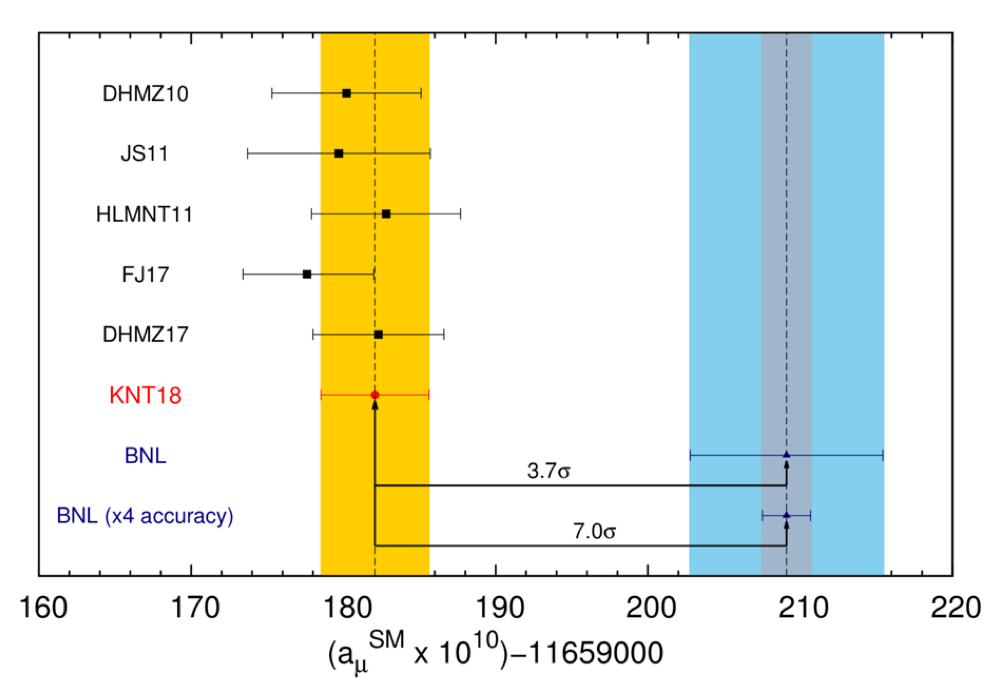
\includegraphics[width=0.9\textwidth]{AlexKPaperComparison}
	\caption[AlexKPaperComparison]{any figures that are directly lifted from someone else's work needs to be cited evertime they're used I believe, even if I cite that work in the text somewhere - \cite{Keshavarzi:2018mgv} }
	\label{fig:AlexKPaperComparison}
\end{figure}



